%
% 公立はこだて未来大学卒業研究中間報告書[全コース対応版]
%
%         ファイル名:"sample.tex"
%
\documentclass[11pt]{ujarticle}
\usepackage{subfig}
\usepackage{funinfosys}
\usepackage{url}
\usepackage[dvipdfmx]{graphicx}

\author{% 
1020259 中村碧\\指導教員 : 松原克弥
}
\course{Intelligent Systems Course}

\title{シームレスなクラウド連携の実現に向けた軽量ロボットソフトウェア基盤mROS 2-POSIXの予備評価}
\etitle{A Preliminary Evaluation of the Lightweight Robot Software Framework mROS 2-POSIX Toward Seamless Cloud Collaboration}
\eauthor{Aoi Nakamura}
\abstract{
ロボットソフトウェア開発において,ROSの利用が増加している.
クラウド連携を用いた分散ロボットシステムの構築が主流だが,ノード配置の柔軟性が課題となっている.
特に,クラウドとロボットのCPUアーキテクチャの違いから,動的なノード再配置が難しい.
先行研究での動的配置機構はオーバーヘッドの増加が問題とされ,mROS 2-POSIXを用いたアプローチも提案されているが,性能評価はint型などのメッセージ型を送受信するアプリケーション上だけで実験されている.
\\ 本研究では,mROS 2-POSIXとROS 2の性能を比較評価する.
実験結果によって得た通信性能やメモリサイズを基に,mROS 2-POSIXが複雑なアプリケーション上でも期待される性能を発揮できることを示す.
}
\keywords{ロボティクス,mROS2-POSIX}
\eabstract{
The use of ROS in robot software development is on the rise. While cloud-integrated distributed robot systems are becoming the norm, there are challenges in the flexibility of node placement. Specifically, the dynamic relocation of nodes is complicated due to differences in CPU architectures between the cloud and robots. Previous research has highlighted the increase in overhead for dynamic placement mechanisms. Although the mROS 2-POSIX approach has been proposed, its evaluation has been limited to applications that send and receive different message types. 
\\ In this study, I evaluate the performance of ROS 2 using mROS 2-POSIX, focusing on communication performance and memory size, to assess mROS 2-POSIX as a lightweight software platform for dynamic placement mechanisms.}
\ekeywords{Roboethics, mROS2-POSIX}
\begin{document}
\maketitle
%\vspace*{-.5cm}

\section{背景と目的}
\label{sec:introduction}
さまざまな産業向けやエンターテイメント関連のロボットシステム,自動車の自動運転技術やIoTシステムの構築においても,これらのソフトウェア開発をサポートするフレームワークとしてRobot Operating System(以下,ROS)の普及が増加している[1].
ROSのプログラミングモデルは,システムの各機能を独立したプログラムモジュール(ノード)として設計することにより,汎用性と再利用性を向上させて,各機能モジュール間のデータ交換を規定することで,効率的かつ柔軟なシステム構築を可能にしている.
たとえば,カメラを操作して周囲の環境を撮影するノード,画像からオブジェクトを識別するノード,オブジェクトのデータを基に動作制御を実行するノードを連携させることで,自動運転車の基本機能の一部を容易に実装できる.
\\ ROSのプログラミングモデルは,ロボット/IoTとクラウドが協力する分散型システムにおいても有効である.
ロボットシステムのソフトウェア処理は,外界の情報を取得する「センサー」,取得した情報を処理する「知能・制御系」,実際に動作するモーターなどの「動力系」の3要素に分類できる[2].
クラウドロボティクス[3]において,主に知能・制御系のノードを高い計算能力を持つクラウドに優先して配置することで,高度な知能・制御処理の実現を促進できる.
さらに,ロボットが取得した情報や状態などをクラウドに集約・保存することで,複数のロボット間での情報共有と利用を容易にする.
一方で,現行のROS実装では,各ノードの配置をシステム起動時に静的に設定する必要があり,クラウドとロボット間の最適なノード配置を事前に設計する必要がある.
しかし,実際の環境で動作するロボットは,ネットワークの状況やバッテリー残量の変動など,システム運用前に予測することが困難な状況変化に対応する必要があり,設定したクラウドとロボット間のノード配置が最適でなくなる可能性がある.
このような状況変化への対応として,ノードを動的に再配置するライブマイグレーション技術があるが,多くの場合でクラウドとロボット間のCPUアーキテクチャが異なり,命令セットがそれぞれ違うため,実行中のノードをシステム運用中にマイグレーションすることは技術的に困難である.
\\ 菅らは,WebAssembly(以下,Wasm)を用いることで,クラウドとロボット間での実行状態を含む稼働中ノードの動的なマイグレーションする手法を実現した[4].
WasmとはWeb上で高速にプログラムを実行するために設計された仮想命令セットアーキテクチャのことで,1つのバイナリが複数のアーキテクチャで動作するため,異種デバイス間でのマイグレーションに適しているといえる.
課題として,ROS 2をWasm化したことでライブマイグレーション後のファイルサイズのオーバーヘッドが増大し,ノードの実行時間が大幅に増えてしまう問題が残った.
柿本ら[5]は,組込みデバイス向けの軽量なROS 2ランタイム実装であるmROS 2-POSIXを採用し,ROSランタイムのWasm化にともなうオーバヘッド増加に対処した.
しかし,採用されたmROS 2-POSIXは指定したメッセージ型をping-pong通信するアプリケーション上でしか評価実験は行われていない[6].そのため,ライブマイグレーション後のオーバーヘッド増加を解決するロボットソフトウェア基盤として,アプリケーションが複雑化した場合の動作が明らかでない.
\\ 本研究では,クラウドとロボット間での実行状態を含む稼働中ノードの動的マイグレーションの実現に向けたmROS 2-POSIXの性能評価を行い,mROS 2がROS 2と比べて動的配置機構ロボットソフトウェア基盤としてどの点で優位性があるのか明らかにすることを目指す.
%目的



\section{mROS2-POSIX}
mROS 2は,ROS 2ノードの軽量実行環境である.
このロボットソフトウェア基盤によって,分散型のロボットシステムへの組込み技術の導入ができる.
組込みデバイスは計算資源が限定的であるが,リアルタイム性の向上および消費電力の削減ができる.
そして,mROS 2がPOSIX[7]に対応したのがmROS 2-POSIXである.
\\ 図1(a)は,mROS 2-POSIXのソフトウェア構成を示す.mROS 2-POSIXアプリケーション層は,ユーザが実装するROS 2ノードに相当する.
\begin{figure}[t]
	\centering
	\begin{minipage}{.5\textwidth}
		\centering
		\subfloat[mROS 2-POSIXの内部構成]{
			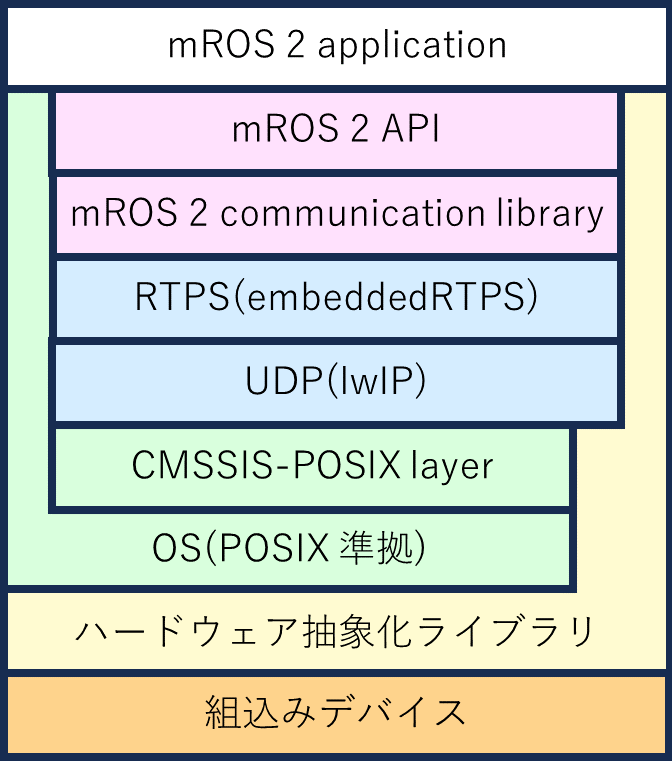
\includegraphics[width=0.35\textwidth]{./src/fig1_mros2posix_a.png}\label{fig:subfig_a}
		}
		\hfill
		\subfloat[mROS 2の内部構成]{
			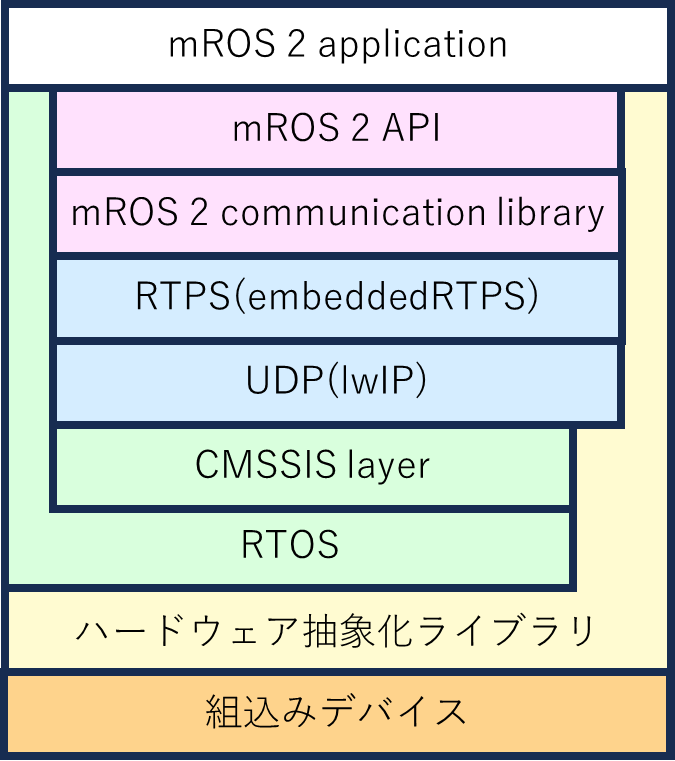
\includegraphics[width=0.35\textwidth]{./src/fig1_mros2_b.png}\label{fig:subfig_b}
		}
	\end{minipage}
	\caption{mROS 2-POSIXとmROS 2のソフトウェア構成}
	
\end{figure}
mROS 2-POSIX API層および通信ライブラリ層は,メッセージを非同期にパブリッシュやサブスクライブするためのコミュニケーションチャネルであるROS 2のTopic[]に相当するAPIおよび通信機能を提供する階層である.
本階層は,ROS 2のネイティブなクライアント通信ライブラリであるrclcppと互換性を保つように設計されている.
mROS 2通信ライブラリでは,rclcppのうちpub/sub通信の基本的な機能のみ実装されている.
利用可能な機能は制限されているものの,組込み技術を導入するROS 2開発者は,汎用OS向けのプログラミングスタイルを踏襲しながらC++によってmROS 2のアプリケーションを実装できる.
\\ Real Time Publish-Subscribe(以下,RTPS)プロトコルスタックにはUDPでパブリッシャとサブスクライバC++実装のembeddedRTPS[8]が採用されている.
\begin{figure}[t]
	\centering
	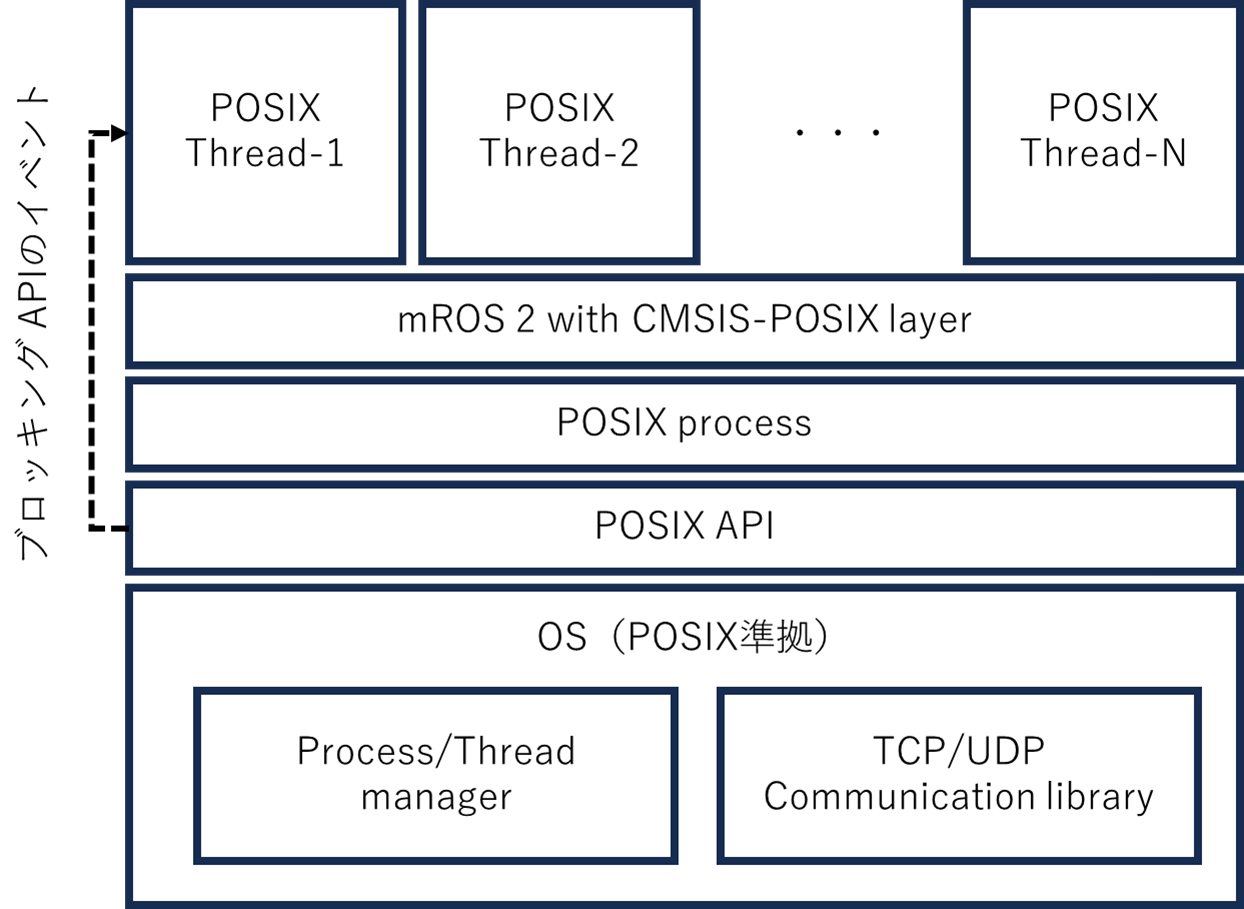
\includegraphics[width=0.6\linewidth]{./src/fig2_execution_structure.png}
	\caption{mROS 2-POSIXの実行方式}
  \label{fig:arch}
\end{figure}
UDPについては組込み向けのC実装であるlwIPが採用されている.
通信層のembeddedRTPSおよびlwIPはCMSAIS-POSIXに依存しており,図1(b)に示すmROS 2のCMSIS-RTOSを互換した層になっている.
最下層にはハードウェアを抽象化したライブラリがある.
\\ mROS 2-POSIXは図2に示す実行方式を採用している.
リアルタイムOSでは,組込みマイコンを実行資源の管理対象として,タスク単位でアプリケーションが実行される.
POSIXにおいてはタスクに相当する概念はプロセスであり,そこから生成されるスレッドを実行単位として処理が進行している.
しかし,mROS 2-POSIXは実行単位であるノードにPOSIXのスレッドを対応づけ,組込みマイコンでの通信処理におけるイベント割込みについては,POSIX準拠OSにおけるブロッキングAPIの発行に相当させて処理している.
% \\ mROS 2とmROS 2-POSIXの機能構造の対応として,タスク管理機能は,スレッドの生成や開始などのPOSIX資源の管理機能に対応付けれている.
% メッセージキューおよびミューテックスによるスレッドの同期・通信および排他制御は,POSIXではPthreadによって対応している.
% メモリ管理機能はAlloc/Freeで,時間管理はOS時刻管理機能で対応している.
% lwIPにおけるUDPパケット処理は,POSIXにおけるOS資源の操作に関する機能で実現されている.

\section{評価方針}
mROS 2-POSIXを評価するにあったって,mROS 2と同様のアプリケーションをROS 2に実装し,比較評価する.
mROS 2-POSIXは,図3のようなハードウェアを通してロボットを制御するアプリケーションの評価は行われていない.
したがって,本研究ではハードウェアを利用してユーザーがロボットを制御するアプリケーションを実装し,mROS 2-POSIXの評価を行う.
評価項目としては,mROS 2-POSIXがROS 2と比べてどの点で優位性があるのかを明らかにするため,以下の項目を設定した.
\begin{itemize}
	\item 通信性能の評価
	\item メモリサイズの評価
\end{itemize}
 通信性能の評価は,ROS 2の基本的な通信機能であるrclcppと第2章でふれたmROS 2-POSIXの通信機能の差異を明確にするために行う.
具体的には,1回の通信をTopicからサブスクライブするまでに要するラウンドトリップタイム(RTT)を計測する.
それを100回行い,その平均と最大値と最小値と標準偏差を取ることで性能比較を行う.
\\メモリサイズの評価は,mROS 2-POSIXの機能構造の対応や,リアルタイム性,消費電力の削減などの特性がメモリ使用量にどのような影響を与えるか検証する.
アプリケーションのバイナリをsizeコマンドで計測しそれぞれプログラムの実行可能コードを格納するtext,初期化済みのグローバル変数と静的変数を格納するdata,初期化されていないグローバル変数と静的変数を格納するbssの3分類を比較する.
%%
%%ハードウェアを通して
%mros2-posixを評価
%ハードウェアを含めたアプリケーションの評価をしてない
%小規模,大規模という話じゃなくて,ハードウェアを通して利用されるアプリケーションの評価をしてないという話にする。
\section{評価アプリケーションの実装}
% Wii Fit BoardとSphero SPRK+を用いたロボット制御アプリケーションは,Wii Fit Boardはユーザの体重移動を検知し,Sphero SPRK+を前後左右に動かすことで,ユーザの体重移動に追従するように動作する.
% 評価アプリケーションの実装として,mROS 2-POSIXとROS 2の両方で同じ機能を持つノードを作成する必要がある.
評価に使用するアプリケーションはSphero SPRK+とWii Fit Boardを用いたロボット制御アプリケーションである.
図3にアプリケーションの構造を示す.
Wii Fit Boardでユーザの体重移動を検知し,Sphero SPRK+を前後左右に動かすことで,ユーザの体重移動に追従するように動作する.
\begin{figure}[t]
	\centering
	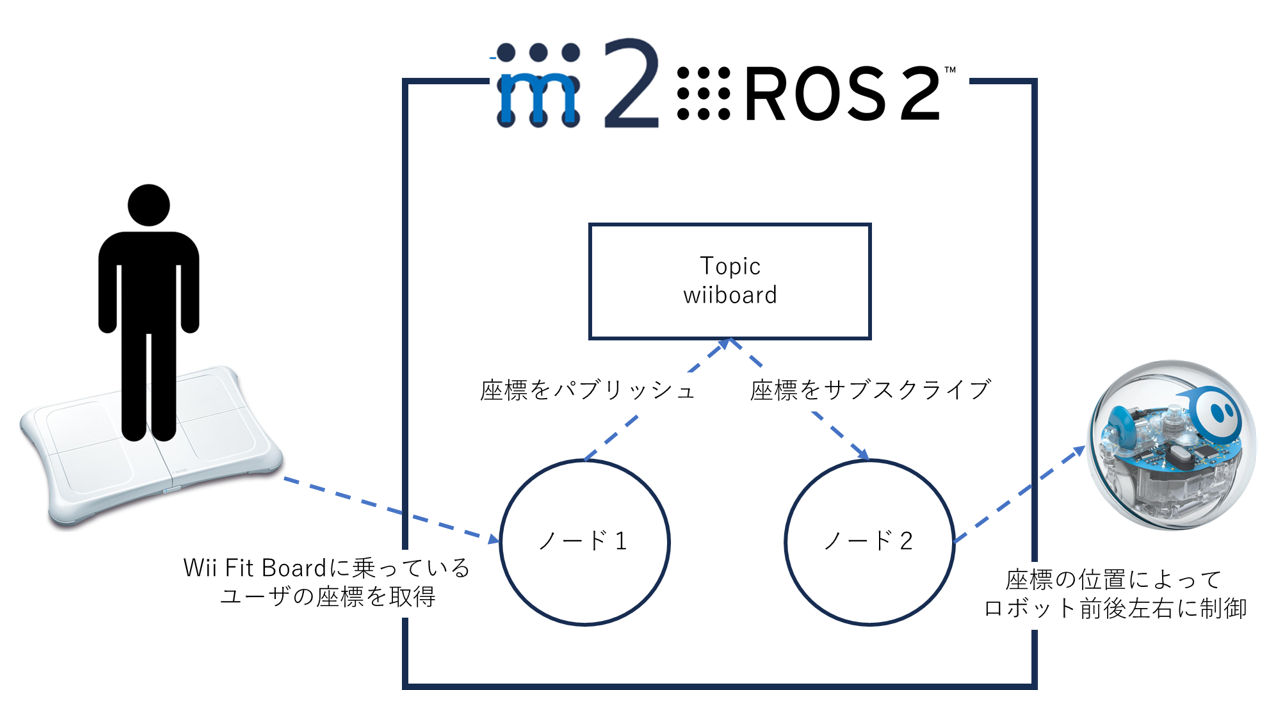
\includegraphics[width=0.7\linewidth]{./src/fig3_application_structure.png}
	\caption{実装するアプリケーション}
  \label{fig:arch}
\end{figure}
アプリケーションは,Wii Fit Boardに乗っているユーザの座標をパブリッシュするノードであると,Wii Fit Boardの座標があるトピックにサブスクライブし,受け取った値をもとにSphero SPRK+を動作させるノードの2つによって実装されている.
ROS 2のアプリケーションは,Wii Fit Boardの値を取得するOSSをROS 2ノード化したものと,Sphero SPRK+を動作させることができるライブラリを提供しているOSSをROS 2ノード化して通信させている.
ROS 2で動作するノードのソースコードはそのまま移植することはできないため,ROS 2のrclcppではなくmROS 2-POSIX固有のAPIを使用して作成する必要がある.
%また,Sphero SPRK+を動作させるライブラリはPythonでコーディングされているため,C++のみに対応しているmROS 2-POSIXではそのまま使用できため,Sphero SPRK+を動作させるライブラリをC++のライブラリに書き換える必要がある.


\section{進捗と計画}
進捗として,アプリケーションはROS 2で動作するノードの作成が完了した.
mROS 2-POSIX対応は未実現である.
mROS 2-POSIXでは,Wii Fit Boardの値をパブリッシュするノードは移植することができた.
Sphero SPRK+のノードの移植は,ライブラリがPythonで書かれているため,C++に書き換える必要があり,現在書き換えに関する検討(調査)を行っている.
%1対
\section{結言}
本研究では,クラウドとロボット間での実行状態を含む稼働中ノードのライブマイグレーションの実現に向けたmROS 2-Posixの評価を行い,mROS 2がROS 2と比べて動的配置機構の実現のソフトウェア基盤としてどの点で優位性があるのか明らかにすることを目指す.
動的配置機構をROS 2環境で実現した手法は,ライブマイグレーション後のファイルサイズのオーバーヘッド増加が課題であるとしている.
課題解決のアプローチとして,ROS 2の軽量ランタイムであるmROS 2-POSIXを採用し,ライブマイグレーション後のオーバーヘッド全体を低減する試みを提案している.
しかし,ROS 2とmROS 2-POSIXの比較評価では,小規模なアプリケーションでしか評価が行われておらず,実際に利用されるようなアプリケーション上での評価は行われていない.
そのため,本研究では,ハードウェアを含めたユーザーがロボットを制御するアプリケーション上でROS 2とmROS 2-POSIXの通信性能やメモリサイズを比較評価し,mROS 2-POSIXを優位性を示す.

\section{知能システムコースにおける本研究の位置づけ}
本研究は,mROS 2-POSIXの評価を行うことで,実行状態を含む稼働中ノードのライブマイグレーションの実現に向けたロボットソフトウェア基盤としての優位性を明らかにすることを目指す過程で,mROS 2-POSIXで動作するロボット制御アプリケーションの実装を行う.
そして,アプリケーションの動作を評価することで,動的配置機構を実装するソフトウェア基盤として適切であるか評価する.
よって,知能システムコースカリキュラムポリシーの「実世界への実装に関する具体的な課題に取り組み,その結果の評価を通じて,新しい方法論や学問領域を切り拓く能力を育む」に該当する.


\begin{thebibliography}{99}
	\bibitem{ros}
	ROSWiki:ROS/Introduction, url{http://wiki.ros.org/ROS/Introduction.}
	\bibitem{robotkenkyuukai}
	ロボット政策研究会: ロボット政策研究会 報告書 ~RT革命が日本を飛躍させる~,\url{https://warp.da.ndl.go.jp/info:ndljp/pid/286890/www.meti.go.jp/press/20060516002/robot-houkokusho-set.pdf (2006).}
	\bibitem{cloudrobotics}
	Kehoe et al. explored cloud-based robot grasping utilizing the Google object recognition engine, presenting their findings in the 2013 IEEE International Conference on Robotics and Automation, pages 4263-4270.
	\bibitem{kan}
	菅文人,松原克弥: クラウドロボティクスにおける異種デバイス間タスクマイグレーション機構の検討,研究報告組込みシステム(EMB),Vol. 2022, No. 36, pp. 1-7(2022).
	\bibitem{kakimoto}
	柿本翔大,松原克弥:クラウド連携を対象としたアーキテクチャ中立なROSランタイムの実現,情報処理学会研究報告, Vol. 2023-EMB-62,No. 51 ,pp. 1-7(2023).
	\bibitem{mROS 2-POSIX hyoukajikken}
	高瀬英希,田中晴亮,細合晋太郎: ロボットソフトウェア軽量実行環境mROS 2のPOSIX対応に向けた実装および評価,日本ロボット学会誌,Vol. 2023-EMB-41,No. 8,pp. 724-727(2023).
	% \bibitem{mROS 2}
	% mROS 2:\url{https://github.com/mROS-base/mros2}
	 \bibitem{POSIX}
	 POSIX:\url{https://www.ibm.com/docs/ja/zos/2.3.0?topic=ulero-posix}
	\bibitem{embeddedRTPS}
	A. Kampmann, et al.: “A Portable Implementation of the Real-Time Publish-Subscribe Protocol for Microcontrollers in Dis-tributed Robotic Applications,” Proc. of ITSC, pp.443–448,2019.
	% \bibitem{lwIP}
	% lwIP Wiki:\url{https://lwip.fandom.com/wiki/LwIP_Wiki}
	% \bibitem{CMSIS-RTOS}
	% CMSIS-RTOS:\url{https://www.keil.com/pack/doc/CMSIS/RTOS/html/index.html}
	% \bibitem{Sphero SPRK+}
	% Sphero SPRK+:\url{https://sphero-edu.jp/teaching/sprk/}
	% \bibitem{Wii Fit Board}
	% Wii Fit Board:\url{https://www.nintendo.co.jp/wii/rfpj/board/index.html}
\end{thebibliography}
\end{document}
%
%
% EOF 
% \\ 図2.1(b)ではmROS 2のソフトウェア構成を示している.
% それぞれCMSIS-RTOS APIに依存しているため,mROS 2-POSIXはPOSIX APIとの差分を吸収する互換層(CMSIS-POSIX layer)を設け,通信を実現している.
% また,mROS 2は実行環境としてリアルタイムOSを採用していることに対し,mROS 2-POSIXではPOSIXに準拠したOS上でpub/sub通信を実現している.
% そのため,リアルタイムOSでは組込みマイコンを実行資源の管理対象として,タスク単位でアプリケーションが実行されるのに対し,POSIXにおいてタスクに相当する概念はプロセスであり,そこから生成されるスレッドを実行単位として処理が進行するという違いがある.
% mROS 2-POSIXでは,図2が示す
% は現時点で,TOPPERS/ASP3カーネル[]およびMbed OS 6[]を用いた実装が公開されている.
% Mbed OS 6は,CMSIS-RTOS APIのレイヤを標準的に備えている一方で,TOPPERS/ASP3カーネルはCMSIS-RTOS APIレイヤを備えていない.
% そのため,mROS 2ではTOPPERS/ASP3カーネル向けの実装として,それぞれのAPI差分を吸収するらっぽそうであるcmsis-asp3を用意して対応されている.
